%----------------------------------------------------------------------------------------
%	PACKAGES AND OTHER DOCUMENT CONFIGURATIONS
%----------------------------------------------------------------------------------------

\documentclass{article}

\usepackage{fancyhdr} % Required for custom headers
\usepackage{lastpage} % Required to determine the last page for the footer
\usepackage{extramarks} % Required for headers and footers
\usepackage[usenames,dvipsnames]{color} % Required for custom colors
\usepackage{graphicx} % Required to insert images
\usepackage{listings} % Required for insertion of code
\usepackage{courier} % Required for the courier font
\usepackage{lipsum} % Used for inserting dummy 'Lorem ipsum' text into the template
\usepackage[utf8]{inputenc}
\usepackage[ngerman]{babel}

% Margins
\topmargin=-0.45in
\evensidemargin=0in
\oddsidemargin=0in
\textwidth=6.5in
\textheight=9.0in
\headsep=0.25in

\linespread{1.1} % Line spacing

% Set up the header and footer
\pagestyle{fancy}
%\lhead{\hmwkAuthorName} % Top left header
\chead{\hmwkClass\ : \hmwkTitle} % Top center head
\rhead{\firstxmark} % Top right header
\lfoot{\lastxmark} % Bottom left footer
\cfoot{} % Bottom center footer
\rfoot{Page\ \thepage\ of\ \protect\pageref{LastPage}} % Bottom right footer
\renewcommand\headrulewidth{0.4pt} % Size of the header rule
\renewcommand\footrulewidth{0.4pt} % Size of the footer rule

\setlength\parindent{0pt} % Removes all indentation from paragraphs

%----------------------------------------------------------------------------------------
%	CODE INCLUSION CONFIGURATION
%----------------------------------------------------------------------------------------

\definecolor{MyDarkGreen}{rgb}{0.0,0.4,0.0} % This is the color used for comments
\lstloadlanguages{Perl} % Load Perl syntax for listings, for a list of other languages supported see: ftp://ftp.tex.ac.uk/tex-archive/macros/latex/contrib/listings/listings.pdf
\lstset{language=Perl, % Use Perl in this example
        frame=single, % Single frame around code
        basicstyle=\small\ttfamily, % Use small true type font
        keywordstyle=[1]\color{Blue}\bf, % Perl functions bold and blue
        keywordstyle=[2]\color{Purple}, % Perl function arguments purple
        keywordstyle=[3]\color{Blue}\underbar, % Custom functions underlined and blue
        identifierstyle=, % Nothing special about identifiers                                         
        commentstyle=\usefont{T1}{pcr}{m}{sl}\color{MyDarkGreen}\small, % Comments small dark green courier font
        stringstyle=\color{Purple}, % Strings are purple
        showstringspaces=false, % Don't put marks in string spaces
        tabsize=5, % 5 spaces per tab
        %
        % Put standard Perl functions not included in the default language here
        morekeywords={rand},
        %
        % Put Perl function parameters here
        morekeywords=[2]{on, off, interp},
        %
        % Put user defined functions here
        morekeywords=[3]{test},
       	%
        morecomment=[l][\color{Blue}]{...}, % Line continuation (...) like blue comment
        numbers=left, % Line numbers on left
        firstnumber=1, % Line numbers start with line 1
        numberstyle=\tiny\color{Blue}, % Line numbers are blue and small
        stepnumber=5 % Line numbers go in steps of 5
}

% Creates a new command to include a perl script, the first parameter is the filename of the script (without .pl), the second parameter is the caption
\newcommand{\perlscript}[2]{
\begin{itemize}
\item[]\lstinputlisting[caption=#2,label=#1]{#1.pl}
\end{itemize}
}

%----------------------------------------------------------------------------------------
%	DOCUMENT STRUCTURE COMMANDS
%	Skip this unless you know what you're doing
%----------------------------------------------------------------------------------------

% Header and footer for when a page split occurs within a problem environment
\newcommand{\enterProblemHeader}[1]{
%\nobreak\extramarks{#1}{#1 continued on next page\ldots}\nobreak
%\nobreak\extramarks{#1 (continued)}{#1 continued on next page\ldots}\nobreak
}

% Header and footer for when a page split occurs between problem environments
\newcommand{\exitProblemHeader}[1]{
%\nobreak\extramarks{#1 (continued)}{#1 continued on next page\ldots}\nobreak
%\nobreak\extramarks{#1}{}\nobreak
}

\setcounter{secnumdepth}{0} % Removes default section numbers
\newcounter{homeworkProblemCounter} % Creates a counter to keep track of the number of problems

\newcommand{\homeworkProblemName}{}
\newenvironment{homeworkProblem}[1][Problem \arabic{homeworkProblemCounter}]{ % Makes a new environment called homeworkProblem which takes 1 argument (custom name) but the default is "Problem #"
\stepcounter{homeworkProblemCounter} % Increase counter for number of problems
\renewcommand{\homeworkProblemName}{#1} % Assign \homeworkProblemName the name of the problem
\section{\homeworkProblemName} % Make a section in the document with the custom problem count
%\enterProblemHeader{\homeworkProblemName} % Header and footer within the environment
}{
%\exitProblemHeader{\homeworkProblemName} % Header and footer after the environment
}

\newcommand{\problemAnswer}[1]{ % Defines the problem answer command with the content as the only argument
\noindent\framebox[\columnwidth][c]{\begin{minipage}{0.98\columnwidth}#1\end{minipage}} % Makes the box around the problem answer and puts the content inside
}

\newcommand{\homeworkSectionName}{}
\newenvironment{homeworkSection}[1]{ % New environment for sections within homework problems, takes 1 argument - the name of the section
\renewcommand{\homeworkSectionName}{#1} % Assign \homeworkSectionName to the name of the section from the environment argument
\subsection{\homeworkSectionName} % Make a subsection with the custom name of the subsection
%\enterProblemHeader{\homeworkProblemName\ [\homeworkSectionName]} % Header and footer within the environment
}{
%\enterProblemHeader{\homeworkProblemName} % Header and footer after the environment
}

%----------------------------------------------------------------------------------------
%	NAME AND CLASS SECTION
%----------------------------------------------------------------------------------------

\newcommand{\hmwkTitle}{Übung\ \#3} % Assignment title
\newcommand{\hmwkDueDate}{Donnerstag,\ 13.\ November\ 2014} % Due date
\newcommand{\hmwkClass}{GPU Computing} % Course/class
\newcommand{\hmwkClassTime}{} % Class/lecture time
\newcommand{\hmwkClassInstructor}{} % Teacher/lecturer
\newcommand{\hmwkAuthorName}{Günther Schindler, Alexander Schapp, Klaus Naumann} % Your name

%----------------------------------------------------------------------------------------
%	TITLE PAGE
%----------------------------------------------------------------------------------------

\title{
\vspace{2in}
\textmd{\textbf{\hmwkClass:\ \hmwkTitle}}\\
\normalsize\vspace{0.1in}\small{Abgabe\ am\ \hmwkDueDate}\\
\vspace{0.1in}\large{\textit{\hmwkClassTime}}
\vspace{3in}
}

\author{\textbf{\hmwkAuthorName}}
\date{} % Insert date here if you want it to appear below your name

%----------------------------------------------------------------------------------------

\begin{document}

\maketitle

%----------------------------------------------------------------------------------------
%	TABLE OF CONTENTS
%----------------------------------------------------------------------------------------

%\setcounter{tocdepth}{1} % Uncomment this line if you don't want subsections listed in the ToC
\newpage
\tableofcontents
\newpage

%----------------------------------------------------------------------------------------
%	Intro
%----------------------------------------------------------------------------------------

\begin{homeworkProblem}[Intro]
Auf einem CUDA-Device gibt es verschiedene Arten von Memory mit je unterschiedlichen
Scope. Die dritten Übung beschäftigt sich mit Global-Memory und dessen Zugriff. 
Global-Memory verwendet den DRAM des CUDA-Device und kann sowohl von Device als auch 
von Host verwendet werden.
\end{homeworkProblem}

%----------------------------------------------------------------------------------------
%	Global Memory - cuda Memcpy
%----------------------------------------------------------------------------------------

\begin{homeworkProblem}[Global Memory - cuda Memcpy]
Als erstes ist die Leistung des Global-Memory-Zugriffs anhand von cudaMemcpy zu testen.
Es soll ein Programm implementiert werden, welches die Leistung von device-to-device
von cudaMemcpy misst.
\\\\
Folgender Quellcodeauschnitt zeigt die Umsetzung dieser Problemstellung. Das long-Array
iItaration enthält 13 Werte für die Memory-Größen 1kb bis 1Gb. Anhand dieser Werte werden
über eine for-Schleife 13 cudaMemcpyDeviceToDevice durchgeführt.
\begin{lstlisting}{c}
  ...
  long iIteration[13] = {1e3, 2e3, 1e4, 2e4, 1e5, 2e5, 1e6, 2e6, 1e7, 2e7, 1e8, 2e8, 5e9};

  /* Run over 13 measurement points */
  for(i = 0; i < 13; i++)
  {
    /* Allocate device memory */
    cudaMalloc(&dmem_a, iIteration[i]*sizeof(char));
    cudaMalloc(&dmem_b, iIteration[i]*sizeof(char));
    ...
    /* Start timer */
    chTimerGetTime(&tsStart);
    /* Start memory copy */
    cudaMemcpy(dmem_a ,dmem_b , iIteration[i]*sizeof(char), cudaMemcpyDeviceToDevice);
    /* Stop timer */
    chTimerGetTime(&tsStop);

    /* Get bandwidth in Byte/sec and print it */
    dBandwidth=chTimerBandwidth(&tsStart, &tsStop, (double) iIteration[i]);

    /* Free allocated device memory */
    cudaFree(dmem_a);
    cudaFree(dmem_b);
  }
  ...
\end{lstlisting}
Nachfolgend ist der Graph für die Messergebnisse dargestellt. X- und Y-Achse sind
logarithmisch aufgetragen. Man kann in der logarithmischen darstellung einen linearen
Verlauf andeuten. Dies deutet auf einen exponentiellen Anstieg der Bandbreite mit
zunehmender Memory Größe hin.
\\\\
Es fällt auf, dass die Messwerte für die Bandbreite sehr den Rahmen der erwarteten
Ergebnisse sprängen. Es wurde eine Bandbreite von ca. 288 GB/s (GDDR5) erwartet.
Speziell der letzte Messwert (bei 1Gb) sticht mit einer gemessenen Bandbreite von 
ca. $ 4 \cdot 10^5 GB$ deutlich hervor.
\\
Eine Erklärung wurde hierfür nicht gefunden.
\begin{center}
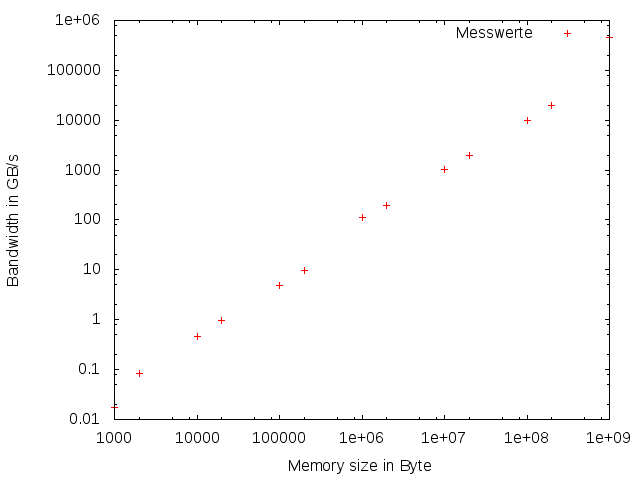
\includegraphics[width=0.7\columnwidth]{../src/part_1/image.png}
\end{center}
\end{homeworkProblem}
\pagebreak
%----------------------------------------------------------------------------------------
%	Global Memory - coalesced thread access
%----------------------------------------------------------------------------------------

\begin{homeworkProblem}[Global Memory - coalesced thread access]
Als nächstes soll die Leistung des Device-Memory-Zugriffs vom Thread-Level gemessen werden.
Es ist ein Kernel zu implementieren der Device-Memory mithilfe von Threads kopiert. Der
Memory-Zugriff soll coalesce ablaufen.
\\\\
Im CUDA-Execution-Model werden Threads in Blöcke gruppiert, welche Multiprozessoren
zugeordnet werden. Während der Ausführung findet eine feinere Gruppierung der Threads in
Warps statt. Multiprozessoren auf der GPU führen Instruktionen für jeden Warp in
SIMD (Single Instruction Multiple Data) Manier aus. Die Warp Größe (praktisch die
SIMD Breite) ist aktuell für alle CUDA fähigen GPUs 32 Threads.
\\\\
Coalesced-Memory-Zugriff bedeutet multiple Memory-Zugriffe in einer einzige Transaktion
zu kombinieren. So kann auf alle aufeinanderfolgenden 128 Bytes 
(32 Single Precision Words) Memory von einem Warp (32 fortlaufende Threads) in einer
einzigen Transaktion zugegriffen werden.
\\\\
In unserem Fall wollen wir ein Integer-Array kopieren was bedeutet, dass wir je 
Warp auf genau 32 Integer-Werte zugreifen können.  
\\\\
Der zur Verfügung gestellte Quellcode muss um die Speicherallokation für Device-Memory
und die Parameterübergabe erweitert werden.
\begin{lstlisting}{c}
  // ...
  cudaMalloc(&d_memoryA, static_cast <size_t> (optMemorySize));
  cudaMalloc(&d_memoryB, static_cast <size_t> (optMemorySize));
  // ...
  globalMemCoalescedKernel<<<grid_dim, block_dim, 0 /*Shared Memory Size*/>>>
                    (d_memoryA, d_memoryB, optMemorySize);
  // ...
\end{lstlisting}
\end{homeworkProblem}
\pagebreak
%----------------------------------------------------------------------------------------
%	Global Memory - thread access with stride
%----------------------------------------------------------------------------------------

\begin{homeworkProblem}[Global Memory - thread access with stride]

\end{homeworkProblem}
\pagebreak
%----------------------------------------------------------------------------------------
%	Global Memory - thread access with offset
%----------------------------------------------------------------------------------------

\begin{homeworkProblem}[Global Memory - thread access with offset]

\end{homeworkProblem}
\pagebreak
\end{document}
